\documentclass[usenames,dvipsnames]{beamer}
\usepackage[orientation=portrait,size=a0,scale=1.4,debug]{beamerposter}
\usepackage{enumitem}
\mode<presentation>{\usetheme{ICRA18}}

% \usepackage[backend=bibtex,maxnames=2]{biblatex}
\usepackage[numbers]{natbib}
\usepackage{booktabs}
\usepackage{moreverb}
\usepackage{url}
\usepackage{multicol,lipsum}
\usepackage{amsmath,amsthm,mathtools}
\usepackage{cuted}
\usepackage{amsfonts}
\usepackage{multirow}
\usepackage{bm}
\usepackage{subfig}
%
\usepackage{algpseudocode}
\usepackage{algorithm}
\usepackage{glossaries}
\usepackage[tight]{units}
\usepackage[normalem]{ulem} % to strike out text, use: \sout{text}
\usepackage{cancel}
\definecolor{Gray}{gray}{0.9}


\usepackage{chemformula}
\usepackage[utf8]{inputenc}
\usepackage[english]{babel} % required for rendering German 
%special 
%characters
\usepackage{siunitx} %pretty measurement unit rendering
\usepackage{ragged2e}
\usepackage[font=scriptsize,justification=justified]{caption}
\usepackage{array,tabularx}

\usepackage{epstopdf}
\usepackage{media9}%
\usepackage{pifont}

% \usepackage{graphics}
\usepackage{graphicx}
\newcommand{\vcenteredinclude}[1]{\begingroup
	\setbox0=\hbox{\includegraphics[width=.8\textwidth, 
	height=.06\paperheight, keepaspectratio]{#1}}%
	\parbox{\wd0}{\box0}\endgroup}
\usepackage[outline]{contour}
% 
\usepackage{calc}


\usepackage{wrapfig}
\newacronym{hyq}{HyQ}{Hydraulically actuated Quadruped}

\newacronym{lf}{LF}{Left-Front}
\newacronym{rf}{RF}{Right-Front}
\newacronym{lh}{LH}{Left-Hind}
\newacronym{rh}{RH}{Right-Hind}

\newacronym{haa}{HAA}{Hip Adduction-Abduction}
\newacronym{hfe}{HFE}{Hip Flexion-Extension}
\newacronym{kfe}{KFE}{Knee Flexion-Extension}

\newacronym{imu}{IMU}{Inertial Measurement Unit}
\newacronym{dofs}{DoFs}{Degrees of Freedom}
\newacronym{rt}{RT}{Real Time}

\newacronym{com}{CoM}{Center of Mass}
\newacronym{cop}{CoP}{Center of Pressure}
\newacronym{zmp}{ZMP}{Zero Moment Point}
\newacronym{icp}{ICP}{Instantaneous Capture Point}
\newacronym{cmp}{CMP}{Centroidal Moment Pivot}
\newacronym{grfs}{GRFs}{Ground Reaction Forces}

\newacronym{ls}{LS}{Least Square}

\newacronym{slip}{SLIP}{Spring Loaded Inverted Pendulum}
\newacronym{eom}{EoM}{Equation of Motions}
\newacronym{qp}{QP}{Quadratic Program}
\newacronym{sqp}{SQP}{Sequential Quadratic Programming}
\newacronym{mic}{MIC}{Mixed-Integer Convex}
\newacronym{cmaes}{CMA-ES}{Covariance Matrix Adaptation Evolution Strategy}
\newacronym{ara}{ARA*}{Anytime Repairing A*}
\newacronym{pca}{PCA}{Principal Component Analysis}
\newacronym{cpg}{CPG}{Central Pattern Generator}
\newacronym{wbc}{WBC}{Whole-Body Control}

\newacronym{mpc}{MPC}{Model Predictive Control}

% SOFT TERRAIN ADAPTATION
\newacronym{awbc}{c$^3$WBC}{Compliant Contact Consistent Whole-Body Control}
\newacronym{swbc}{sWBC}{Standard Whole-Body Control}
\newacronym{c3wbc}{c$^3$WBC}{Compliant Contact Consistent Whole-Body Control}
\newacronym{ste}{TCE}{Terrain Compliance Estimator}
\newacronym{c3}{\texttt{c}$^3$}{compliant contact consistent}

\newacronym{stance}{STANCE}{Soft Terrain Adaptation aNd Compliance Estimation}

\newacronym{wbopt}{WBOpt}{Whole-Body Optimization}


\newacronym{hc}{HC}{Hunt and Crossley's}
\newacronym{kv}{KV}{Kelvin-Voigt's}

\newacronym{wllsr}{WLLSR}{Weighted Linear Least Squared Regression}

\newcommand{\grfs}{\gls{grfs}~}

\newacronym{mae}{MAE}{Mean Absolute Tracking Error}

\newacronym{ode}{ODE}{Open Dynamics Engine}
\newcommand{\reducespace}{\vspace{-1.5em}}
%\newcommand{\reducespace}{\vspace{0em}}
\newcommand{\Rnum}{\mathbb{R}} % Symbol fo the real numbers set
\newcommand{\hf}{\textsc{hf}}
\newcommand{\vect}[1]{\mathbf{#1}} %vector bold

\newcommand{\grf}{F_{\mathrm{grf}}} % vector to denote the contact forces, ground reaction forces
\newcommand{\grfp}[1]{F_{\mathrm{grf,#1}}} % vector to denote the contact forces, ground reaction forces
\newcommand{\grfest}[1]{\hat{F}_{\mathrm{grf},#1}} % vector to denote the contact forces, ground reaction forces

\newcommand{\mrm}[1]{\mathrm{#1}}
\newcommand{\nmrm}[1]{{#1}}
\newcommand{\fratop}[2]{\genfrac{}{}{0pt}{}{#1}{#2}}
\newcommand{\mx}[1]{\mathbf{\bm{#1}}} 				% Matrix symbol
%\newcommand{\vc}[1]{\mathbf{\bm{#1}}} 					% Vector symbol
\newcommand{\vc}[1]{#1}
\newcommand{\degree}{\ensuremath{^\circ}}				% define the degree symbol
\newcommand{\pder}[2]{\frac{\partial#1}{\partial#2}}		% partial derivative
\newcommand{\refframe}[1]{\mbox{\textless#1\textgreater}}	% to denote a reference frame
\DeclareMathOperator*{\argmin}{\arg\!\min}				% argmin
\DeclareMathOperator*{\argmax}{\arg\!\max}				% argmax
\DeclareMathOperator*{\st}{s.t.}						% subject to
\DeclareMathOperator*{\dif}{\mathrm{d}}					% d
\DeclareMathOperator*{\half}{\frac{1}{2}}					% one half
\newcommand{\mat}[1]{\ensuremath{\begin{bmatrix}#1\end{bmatrix}}}	% matrix
\newcommand{\rank}[1]{\text{rank}(#1)}							% rank
\newcommand{\diag}[1]{\text{diag}(#1)}							% diag
\newcommand{\x}{\ensuremath{\times}}
\newcommand{\dx}[1]{\ensuremath{\delta x_{#1}}}					% dx
\newcommand{\du}[1]{\ensuremath{\delta u_{#1}}}					% du
\newcommand{\DX}[0]{\ensuremath{\Delta X}}						% DX
\newcommand{\DU}[0]{\ensuremath{\Delta U}}						% DU
\newcommand{\ith}[0]{\ensuremath{i^\text{th}}}					% i-th
\newcommand{\T}[0]{\ensuremath{\top}}							% transpose symbol
%\newcommand{\Rv}[1]{\ensuremath{\mathbb{R}^{#1}}}				% set of real-valued vectors
%\newcommand{\R}[2]{\ensuremath{\mathbb{R}^{#1\times #2}}}		% set of real-valued matrices
\newcommand{\Spd}[1]{\ensuremath{\mathbb{S}_+^{#1}}}			% set of symmetric positive-definite matrices
\newcommand*\rfrac[2]{{}^{#1}\!/_{#2}}%running fraction with slash - requires
% math mode.

\newcommand{\crossmx}[1]{\mat{#1}_{\times}} %vector bold

\newcommand\bovermat[2]{\makebox[0pt][l]{$\smash{\overbrace{\phantom{%
    \begin{matrix}#2\end{matrix}}}^{\text{#1}}}$}#2}


\newcolumntype{Z}{>{\centering\arraybackslash}X} % centered tabularx columns
\sisetup{per=frac,fraction=sfrac}

\newcommand{\bmcolor}[1]{\textcolor{RoyalBlue}{\bm{#1}}}

\title{WoLF: the Whole-body Locomotion Framework for Quadruped Robots}



\author{\normalsize Gennaro Raiola, Michele Focchi,Enrico Mingo Hoffman}
\institute[]{\textcolor{black}{
		Universit\`a di Trento, Via Sommarive, 9, 38123 Trento, Italy\\		
		Istituto Italiano di Tecnologia (IIT), Italy.\\
		PAL Robotics, Carrer de Pujades 77, 08005 Barcelona, Spain}}


\linespread{1.05}
\begin{document}
\begin{frame}       \vspace{30pt}
\begin{columns}

\begin{column}{.494\textwidth}
\begin{myblock}{{\large Introduction}}
	

\textbf{Motivation:}\\
 the Search and Rescue Robots Market is projected to grow with a Compound Annual Growth Rate (CAGR) of more than 20\%\footnote{\url{https://www.mordorintelligence.com/industry-reports/search-and-rescue-robots-market}}.
 Allied Market Research, reported that the global inspection,  and surveillance robots market generated \$940 million in 2020 and is expected to reach close to \$14 billion by 2030\footnote{\url{https://www.cnbc.com/2021/12/26/robotic-dogs-taking-on-jobs-in-security-inspection-and-public-safety-.html}}.	\\
	
	
\textbf{Problem:}\\
\begin{itemize}
	\setlength{\itemindent}{-10pt}
	\item lack of textit{generic} and \textit{robot agnostic} control software solutions to control quadruped robots
	\item  absence of a common and standardized software framework, high level of expertise required to control such platforms,
	\item   increased Complexity  when the quadruped robots are equipped with one (or more) manipulator(s)
\end{itemize}
\vspace{20pt}
	
\textbf{Solution:} Wolf
\begin{figure}[thb!]
	\centering
	
\includegraphics[width=0.5\columnwidth, trim={7cm 5.5cm 7cm 5.5cm}, clip=true]{images/wolf-logo.pdf}
	\label{fig:wolf_logo}
\end{figure}

\vspace{20pt}
\textbf{In more details:}\\
\begin{itemize}
	\setlength{\itemindent}{-10pt}
	\item   end-to-end software suite devoted to the loco-manipulation of quadruped robots. 
	\item abstracts the complexity of planning and control of quadrupedal robot hardware 
	\item allows multiple tele-operation devices
	\end{itemize}
\end{myblock} 







\begin{myblock}{\large WoLF objectives} 

\begin{figure}
	\centering
	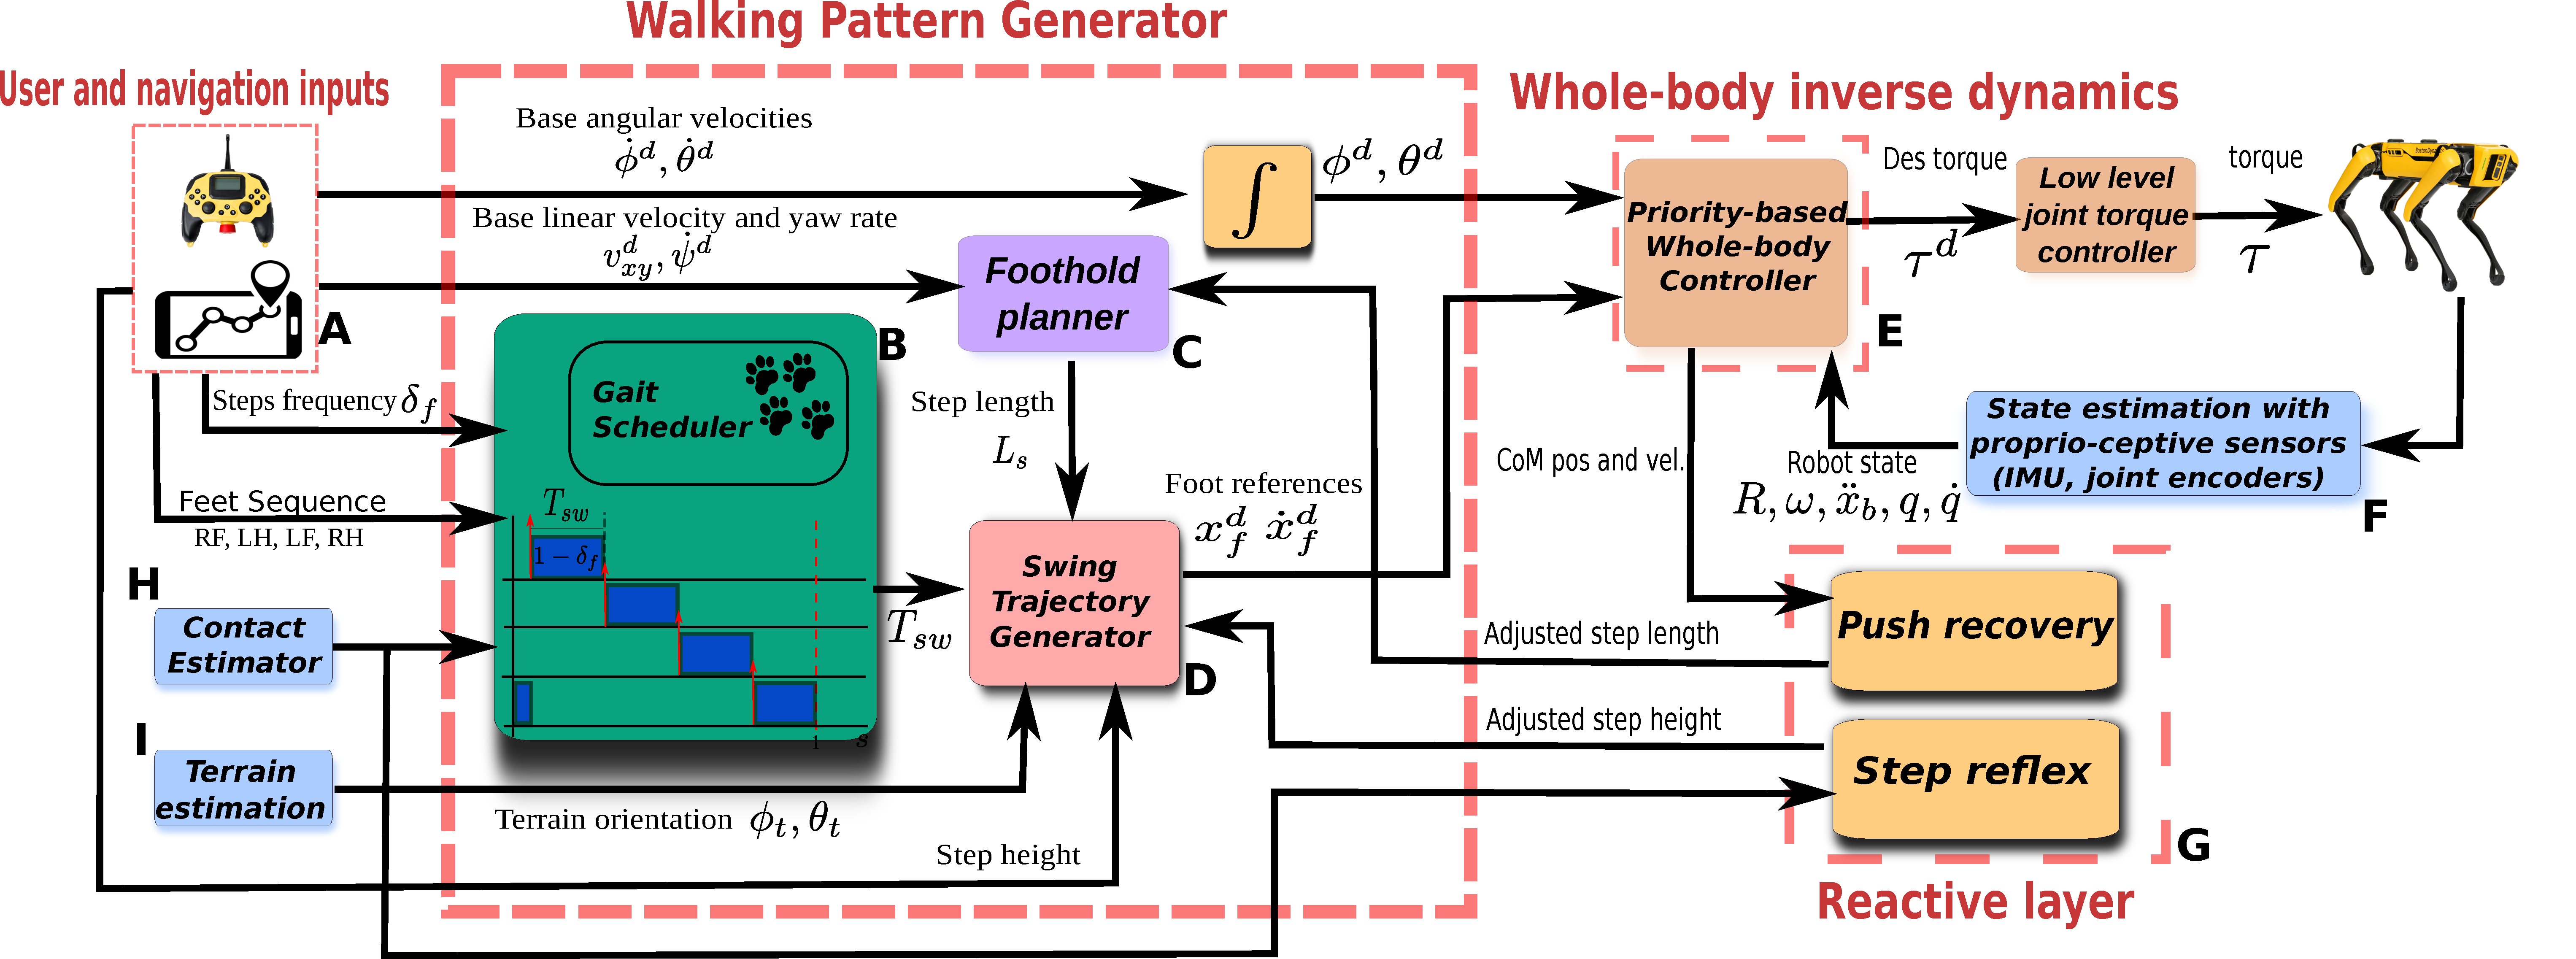
\includegraphics[width=\textwidth]{images/block_diagram_updated.pdf}
	\caption{WoLF block diagram overview. The diagram is composed of four logical layers: the user and navigation input layer, the walking pattern generator, the whole-body inverse dynamics, and the reactive layer. Each layer is composed of one or more components. A description of the layers and their components is detailed in Section~\ref{sec:components}.\textcolor{red}{simplify this or put full page} }
	\label{fig:diagram}
\end{figure}


\textbf{Features:}
\begin{itemize}
	\item plug-and-play software framework, easy to tune 
	\item  adaptable to any quadruped robot without the need for specific knowledge about locomotion or control.	
	\item promote strandardization: use of established robotics tools and technologies such as ROS~\cite{quigley2009ros}, Gazebo~\cite{agueroVRC2015}, OpenSoT~\cite{hoffmanOpenSoT2017} 	
	\item  Differently from CHAMP, WoLF features support for on-board manipulators.
	\item extend the capabilities of quadrupedal platforms with manipulation and navigation skills.
\end{itemize}

\textbf{How is it done?}\\
\vspace{20pt}
The WoLF project started from the work in~\cite{raiola2020} about a novel locomotion framework for quadrupedal robots. 
We designed it to work as a plugin for ros\_control \cite{chitta2017ros_control}. The ros\_control package permits to easily abstract the particular hardware for both the quadruped and/or the manipulator and therefore to re-use the same controller with different robots provided that they expose an effort interface.


\end{myblock}




\begin{myblock}{\large Wolf components}
	
	%\begin{columns}
	%\begin{column}{0.63\textwidth}
	
	\textbf{How is it done?}\\
	\begin{itemize}
		\item User inputs and navigation
		\item Walking pattern generator and reactive layer
		\item State and Terrain Estimation
		\item Whole-Body Inverse Dynamics
	\end{itemize}
	%\end{column}
	%\begin{column}{0.3\textwidth}
	%\begin{figure}[tb]
	%	\centering
	%	\includegraphics[width=0.9\columnwidth]{figures/model.pdf}
	%\end{figure}
	%\end{column}	
	%\end{columns}	
\end{myblock}

\end{column}

\begin{column}{.494\textwidth}
\begin{myblock}{\large Software Packages}

	\begin{figure}[thb!]
		\centering
		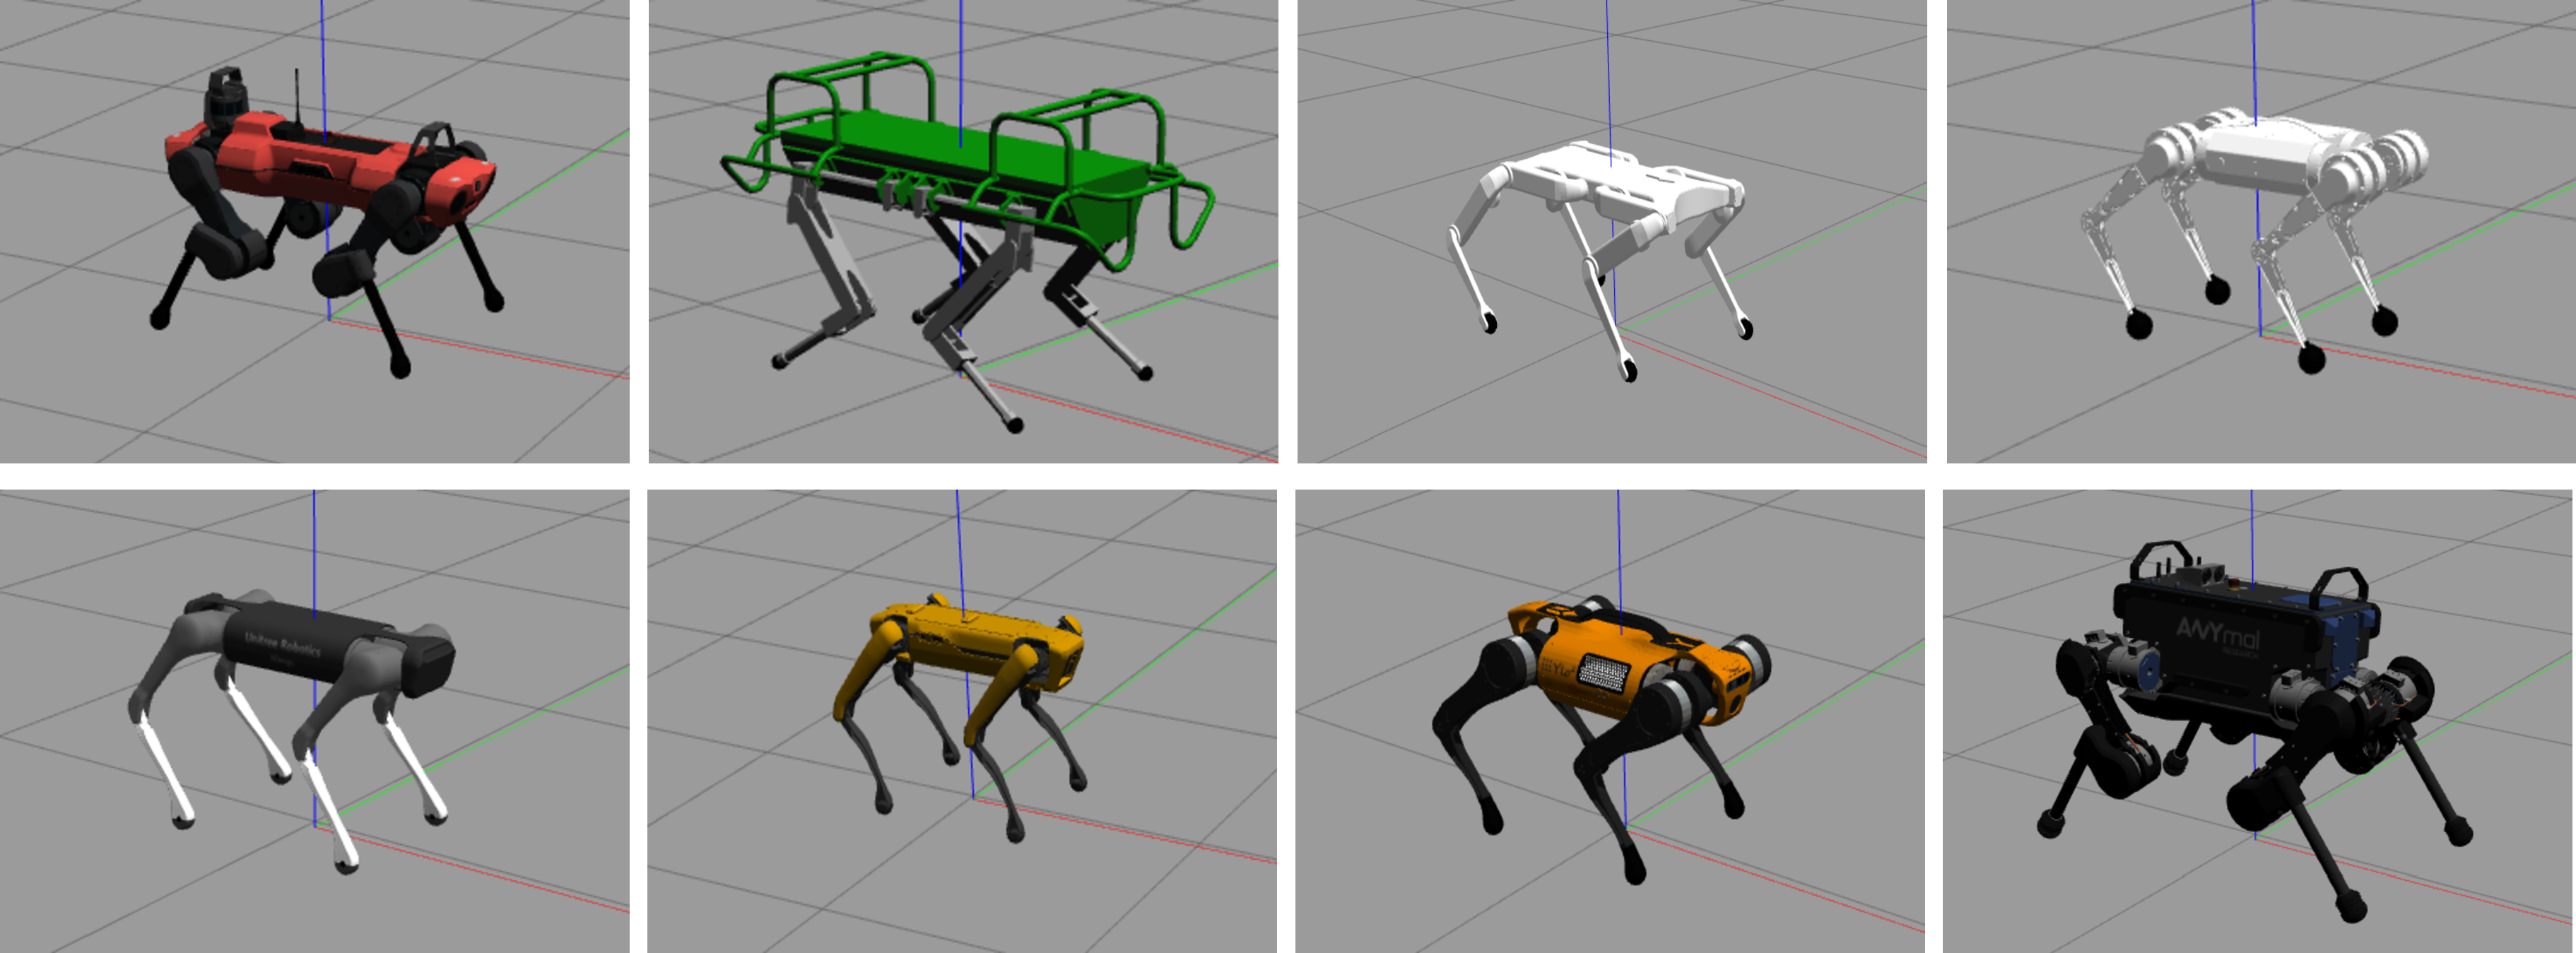
\includegraphics[width=0.8\columnwidth]{images/all_robots.pdf}
		\caption{Robots currently supported in simulation by WoLF. From top-left to bottom-right: AnymalC, HyQ, Solo, Minicheetah, Aliengo, Spot\textsuperscript\textregistered \ , Ylo2, Anymal.}
		\label{fig:robots}
	\end{figure}
	
	The various WoLF packages are hosted on Github. The entry point to set up and run WoLF on any Ubuntu PC is its setup package\footnote{\url{https://github.com/graiola/wolf-setup}}. The other packages are:
	\begin{itemize}
		\item wolf\_descriptions% \footnote{\url{https://github.com/graiola/wolf_descriptions}}
		: it contains robot and sensor descriptions used within the framework (Figure~\ref{fig:robots}). It is possible to use this package to add and try new robots.
		\item wolf\_gazebo\_resources%\footnote{\url{https://github.com/graiola/wolf_gazebo_resources}}
		: it contains Gazebo models and other resources to adapt and create customized simulation environments.
		\item wolf\_hardware\_interface%\footnote{\url{https://github.com/graiola/wolf_hardware_interface}}
		: it implements the hardware interface for ros\_control to be used with WoLF.
		\item wolf\_gazebo\_interface%\footnote{\url{https://github.com/graiola/wolf_gazebo_interface}}
		: This is the Gazebo hardware interface for ros\_control.
		\item wolf\_aliengo\_interface%\footnote{\url{https://github.com/graiola/wolf_aliengo_interface}}
		: Aliengo hardware interface for WoLF. 
		\item wolf\_ylo2\_interface% \footnote{\url{https://github.com/graiola/wolf_ylo2_interface}}
		: Ylo2 hardware interface for WoLF.
		\item wolf\_navigation% \footnote{\url{https://github.com/graiola/wolf_navigation}}
		: This package is used to provide navigation capabilities to WoLF. It integrates and provides several utilities such as odometry computation, way-point definition, and so on.
	\end{itemize}
\end{myblock}	
	
	
\vspace{-20pt}	
\begin{myblock}{\large Applications} 
	%
Applications range from nuclear decommissioning to mining, search \& rescue, inspection, and surveillance. In addition, this technology can be applied to help human workers
in order to reduce labor accidents, as well as in elderly
care and space exploration. The main focus for most end-users is the ability to operate either autonomously or semi-autonomously, through tele-operation.
%	
\begin{figure}[thb!]
	\centering
	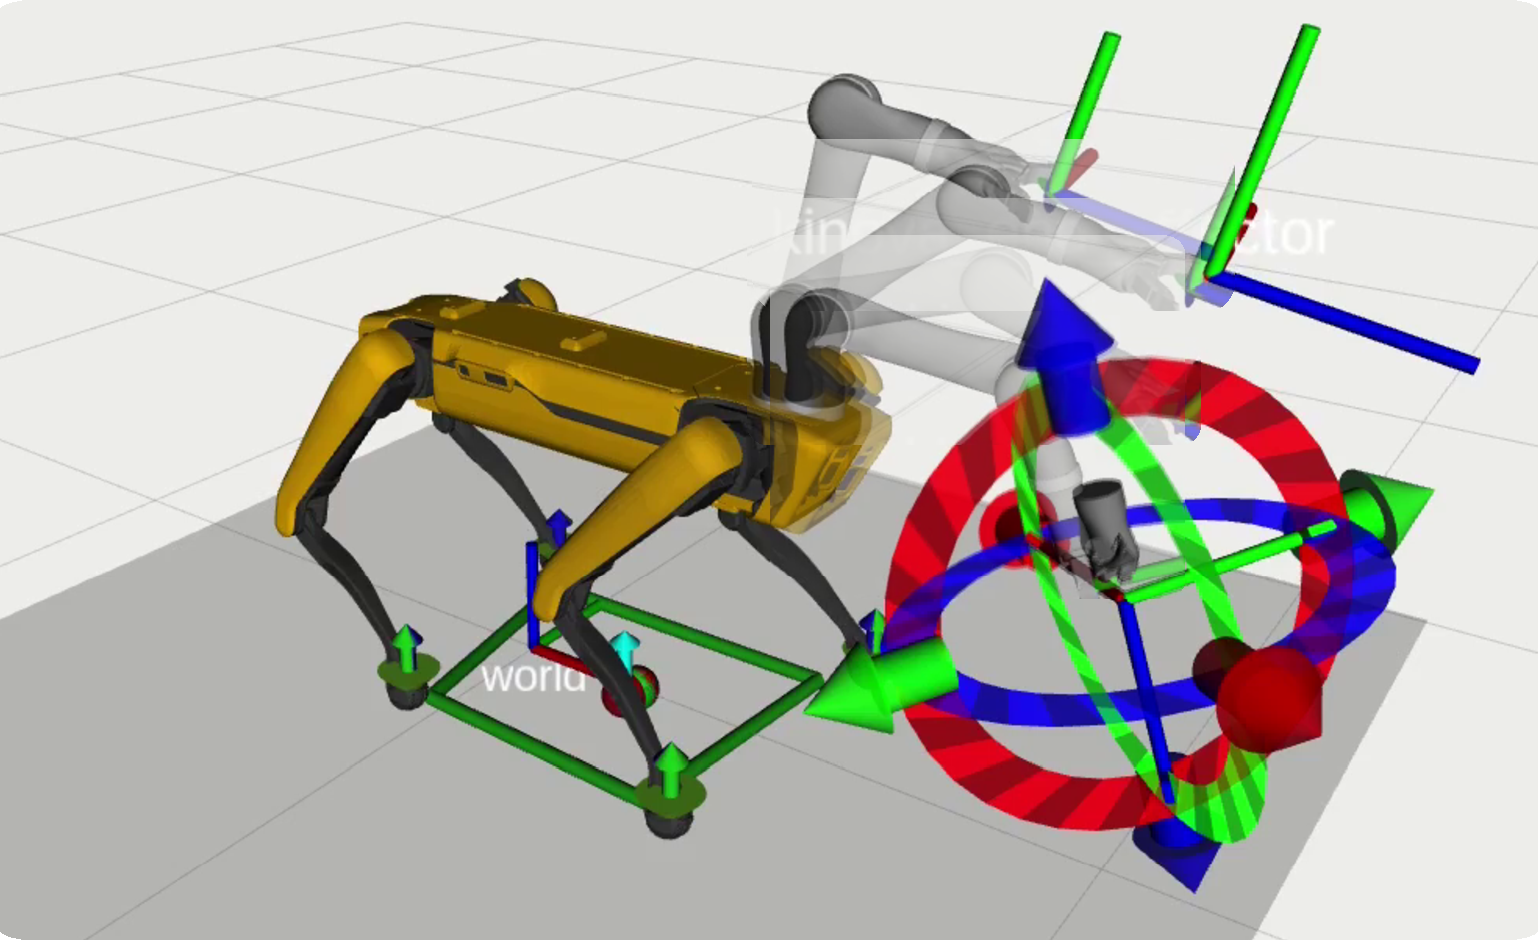
\includegraphics[width=0.5\columnwidth]{images/spot_arm.pdf}
	\caption{Spot\textsuperscript\textregistered \  with a kinova manipulator mounted on its base. WoLF permits to easily combine quadruped platforms with different robotic manipulators. In this example, the kinova end-effector is tele-operated with a ROS interactive marker.}
	\label{fig:spot_arm}
\end{figure}
%
%In this section, we list some of the possible applications of the framework to use cases that are nowadays of increasing interest for the end-users. 
%
\begin{figure}[thb!]
	\centering
	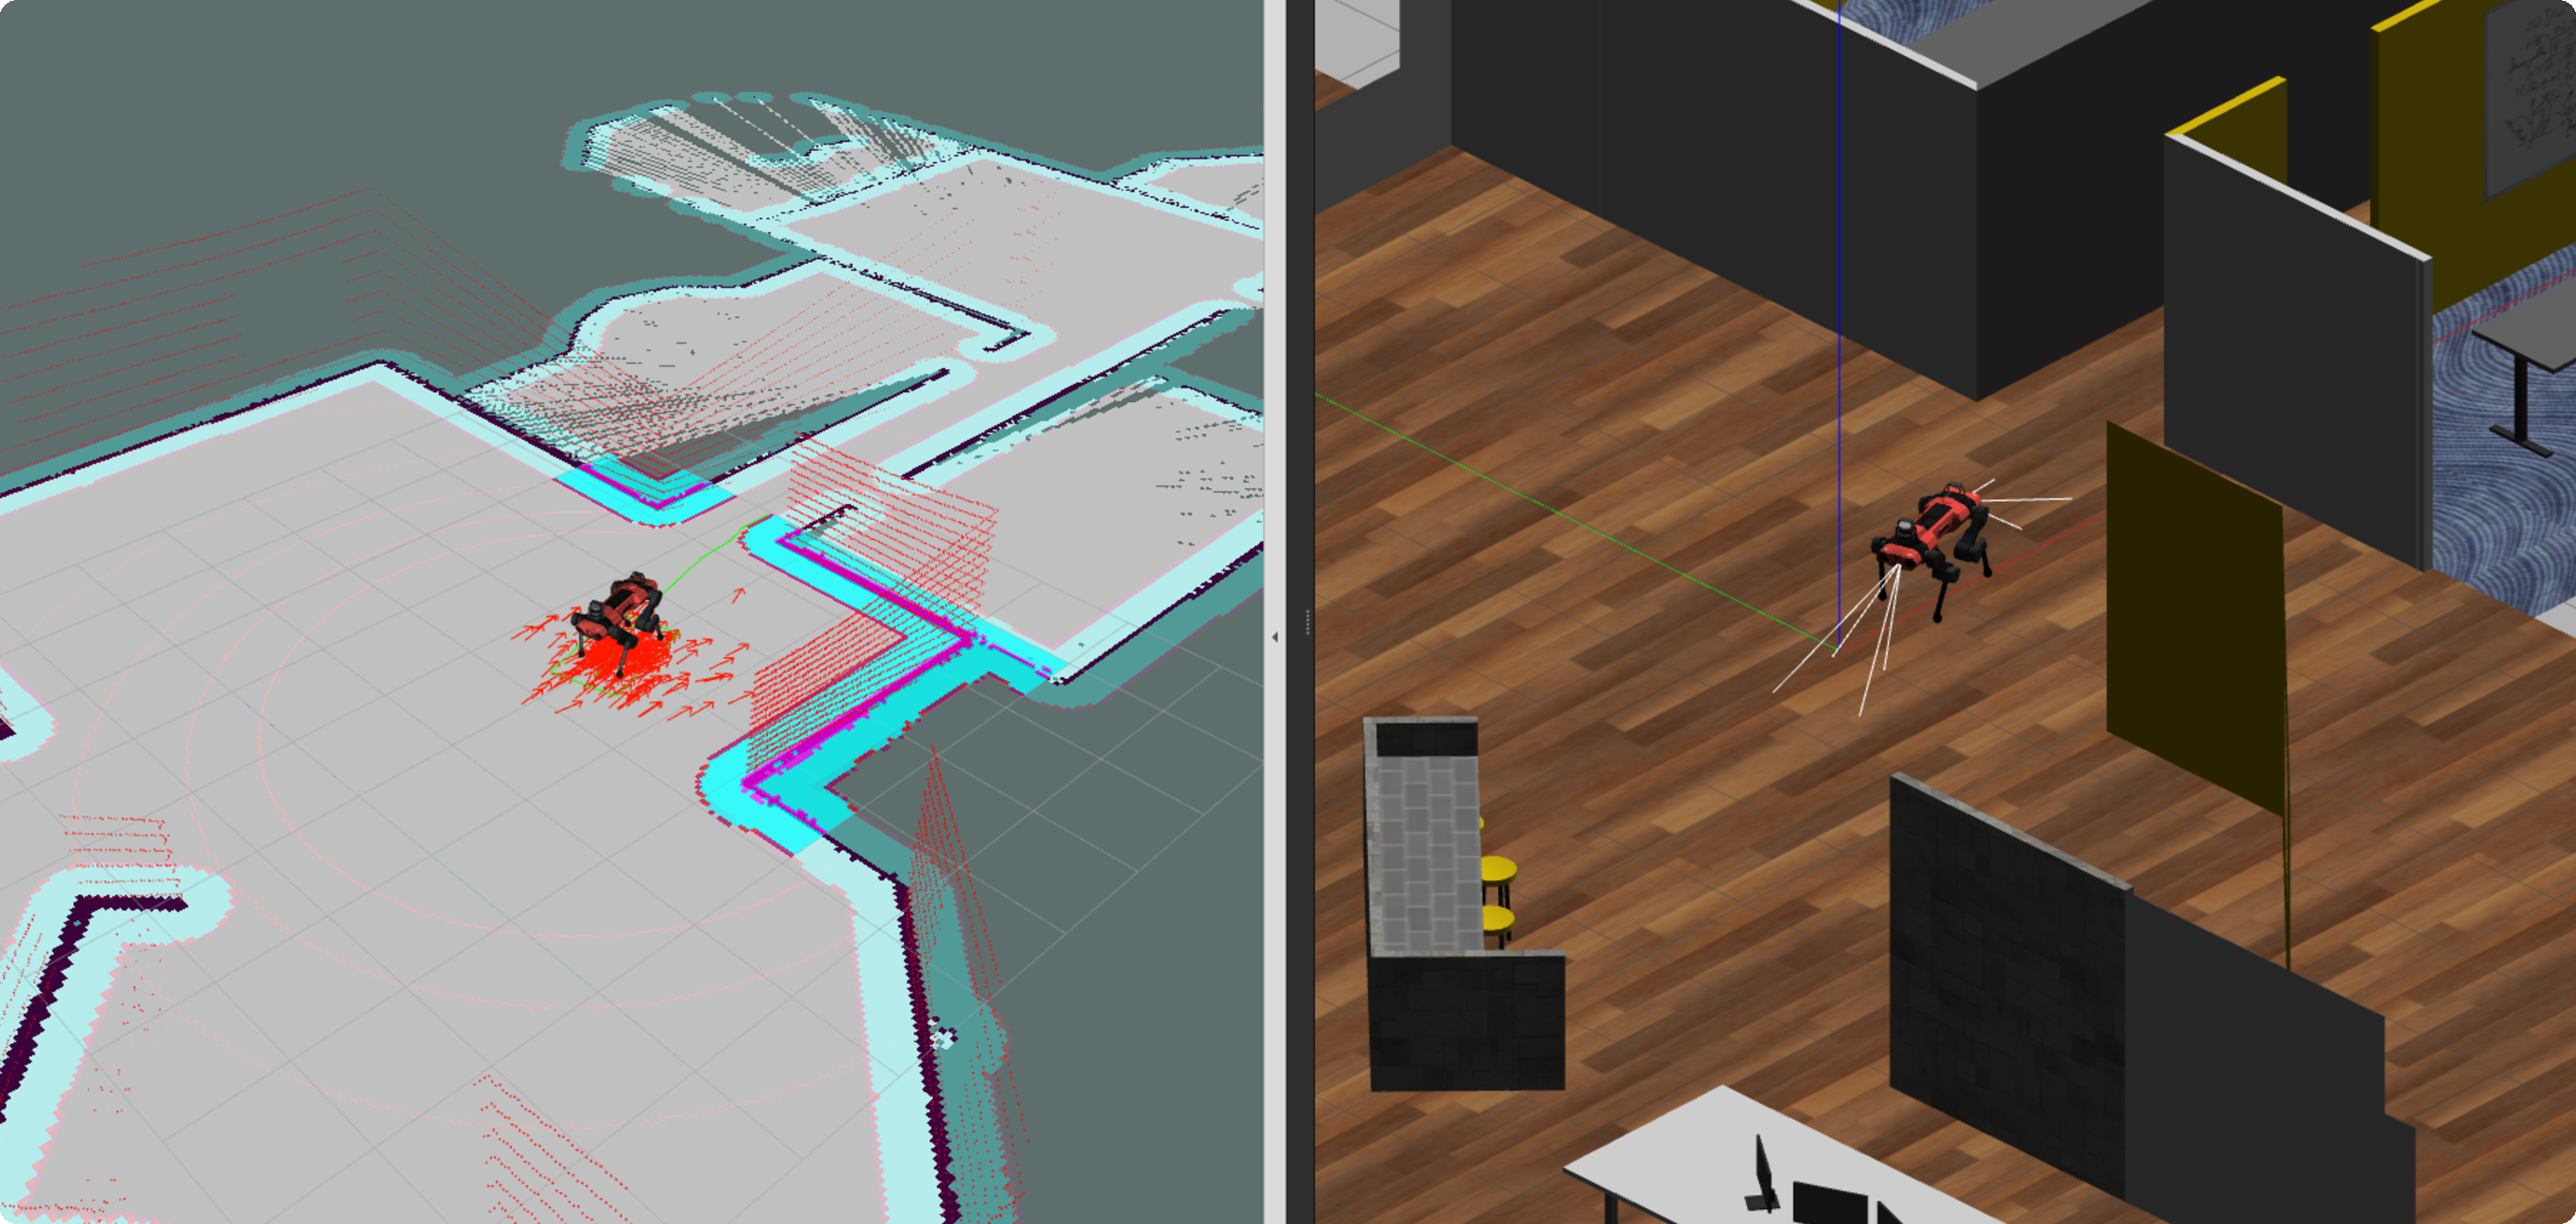
\includegraphics[width=0.5\columnwidth]{images/anymalc_navigation.pdf}
	\caption{AnymalC navigating and reconstructing the map in simulation scenario.}
	\label{fig:anymalc_navigation}
\end{figure}
%
\end{myblock}

%\vspace{-20pt}
\begin{myblock}{{\large Conclusions}}
\begin{itemize}

	\item WoLF provides a plug-and-play software framework easy to tune and adaptable to any quadruped robot without the need for specific knowledge about locomotion or control.
	\item It promote strandardization: use of established robotics tools and technologies such as ROS Gazebo, OpenSoT.
	\item It extend the capabilities of quadrupedal platforms with manipulation and navigation skills.

\end{itemize}
	
\end{myblock} 

\vspace{-20pt}
\begin{myblock}{\large References}
	\linespread{0.9}
	\scriptsize
\begin{thebibliography}{10}
	\providecommand{\url}[1]{#1}
	\csname url@samestyle\endcsname
	\providecommand{\newblock}{\relax}
	\providecommand{\bibinfo}[2]{#2}
	\providecommand{\BIBentrySTDinterwordspacing}{\spaceskip=0pt\relax}
	\providecommand{\BIBentryALTinterwordstretchfactor}{4}
	\providecommand{\BIBentryALTinterwordspacing}{\spaceskip=\fontdimen2\font plus
		\BIBentryALTinterwordstretchfactor\fontdimen3\font minus
		\fontdimen4\font\relax}
	\providecommand{\BIBforeignlanguage}[2]{{%
			\expandafter\ifx\csname l@#1\endcsname\relax
			\typeout{** WARNING: IEEEtran.bst: No hyphenation pattern has been}%
			\typeout{** loaded for the language `#1'. Using the pattern for}%
			\typeout{** the default language instead.}%
			\else
			\language=\csname l@#1\endcsname
			\fi
			#2}}
	\providecommand{\BIBdecl}{\relax}
	\BIBdecl
	

	\bibitem{TODO}
	S.~Fahmi et al., Passive whole-body control for quadruped robots: Experimental validation over challenging terrain, RA-L 2019.
	
	
\end{thebibliography}
\end{myblock}%\vfill

\end{column}


\end{columns}
\end{frame}
\end{document}
